\chapter{Propuesta y desarrollo de la solución}

Los números de este capítulo salen de la corrida del 6 de noviembre de 2026. Quedó firmada en \texttt{results/matching/oe1\_firma.json} (fecha \texttt{2026-11-06T21:00:02Z}). El código que hoy permite repetirla está en \url{https://github.com/denniskano/piloto-bank-api-bian}, commit \texttt{12c1c04}. No recalculamos los scores el 21 de noviembre.

\section{Presentación de la propuesta de solución}

El objetivo general pide un número por par contrato $\times$ dominio. La propuesta es un prototipo con cuatro programas. Cada uno lee la salida del anterior.

\begin{enumerate}
  \item \path{python -m ofb_bian.procesar_openapi} lee los YAML y escribe \path{results/consolidado/}. Esos CSV no van a GitHub. Se regeneran.
  \item \texttt{python -m ofb\_bian.matching\_v0} arma los pares de I1 a I6 y calcula E, el S léxico y C.
  \item \texttt{python -m ofb\_bian.matching\_s1} recalcula solo S, con MiniLM, sobre los pares que congeló el paso anterior. E y C no se tocan.
  \item \texttt{python -m ofb\_bian.mapa\_ofb\_bian} es un catálogo extra (préstamos, tarjetas, inversiones). No entra en $n = 7$.
\end{enumerate}

No corrimos las 38 APIs contra los 258 dominios. No hay YAML de un banco emisor. No entrenamos un clasificador.

\begin{table}[ht]
  \centering
  \caption{Qué quedó hecho el 6 de noviembre de 2026, por objetivo}
  \label{tab:oe}
  \small
  \begin{tabular}{@{}p{0.22\textwidth}p{0.40\textwidth}p{0.28\textwidth}@{}}
    \toprule
    Objetivo & Hecho & Falta \\
    \midrule
    OE1. Normalizar & Parser sobre 296 YAML. Firma 296/296. & El parser no aplana \texttt{allOf}. \\
    OE2. Estructural & Greedy uno a uno en I1--I6. Pares congelados. & Etiquetas de un lector. \\
    OE3. Semántico & S léxico y S MiniLM sobre esos pares. & No hay etiquetas para un ajuste. No lo hacemos. \\
    OE4. Integrar & AlignmentScore $= (S+E+C)/3$ y el nivel. & Precision, recall, F1 y kappa. \\
    \bottomrule
  \end{tabular}
\end{table}

\begin{figure}[ht]
  \centering
  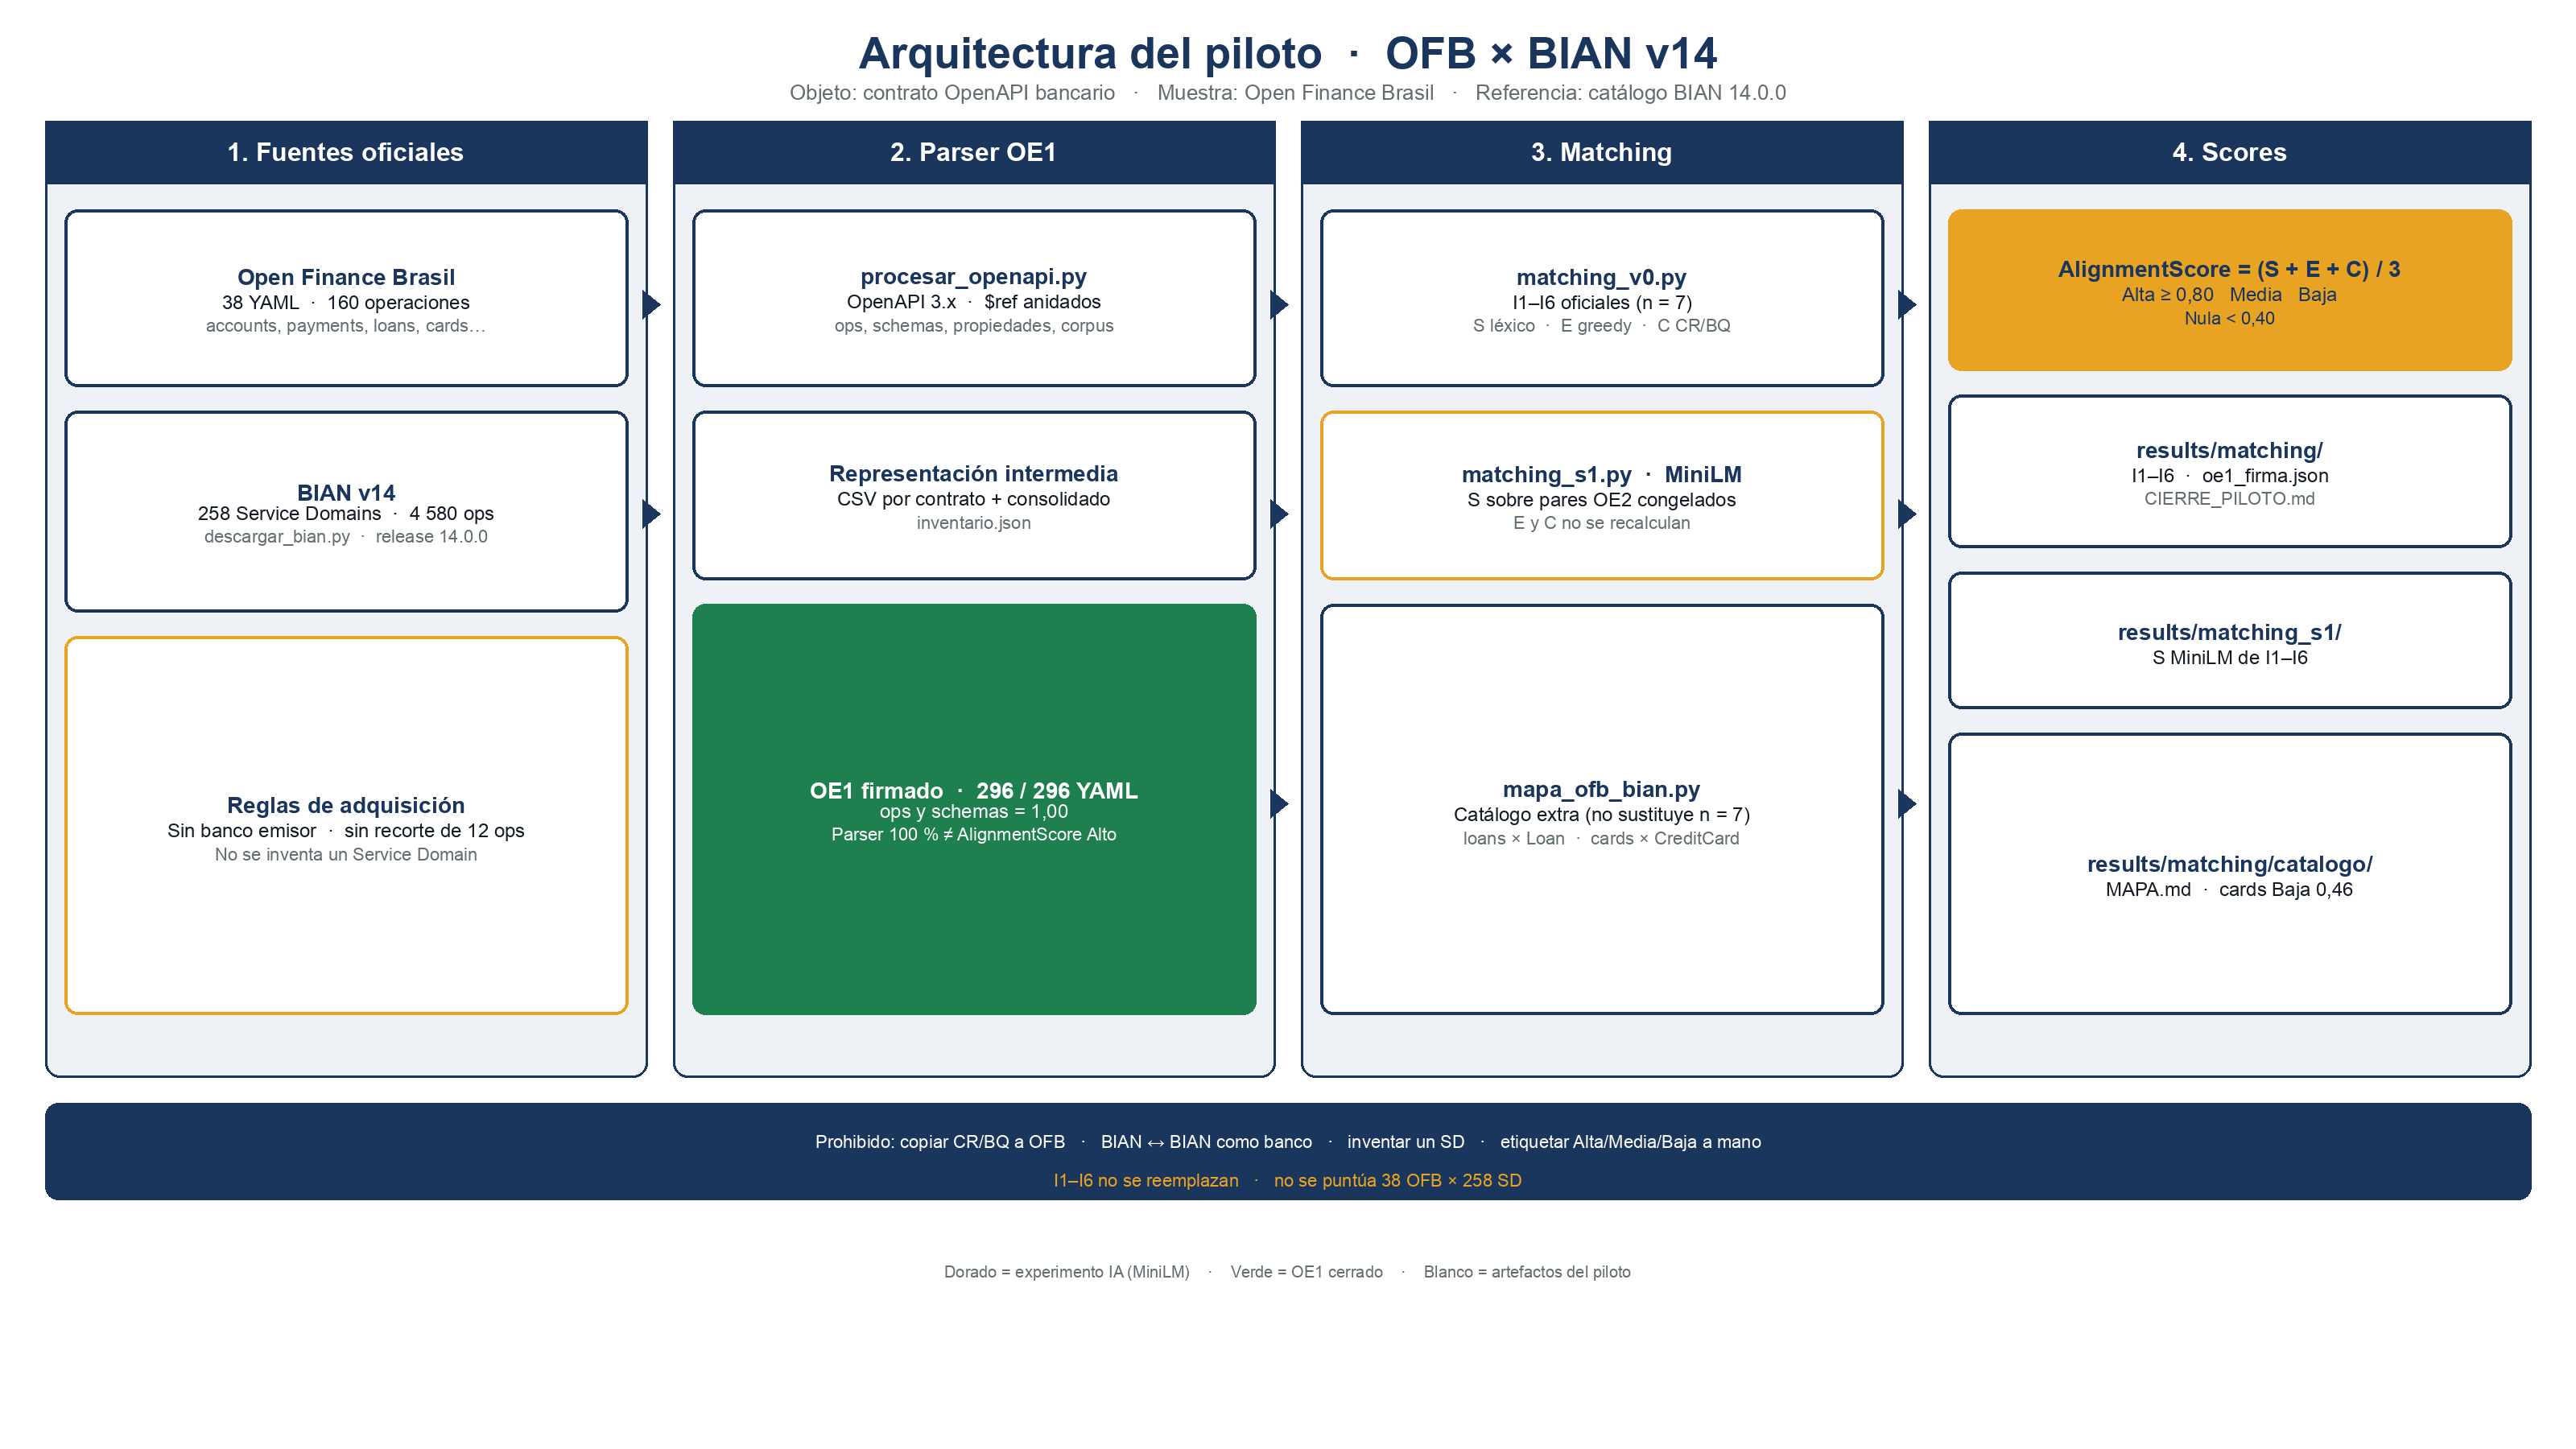
\includegraphics[width=\textwidth]{arquitectura-piloto}
  \caption{Pipeline que ya corrió sobre Open Finance Brasil. El corpus de la tesis es más ancho. Esos YAML todavía no pasan por estas cajas}
  \label{fig:arquitectura}
\end{figure}

\section{Desarrollo de la propuesta de solución}

\subsection{Datos}

La población sigue siendo cualquier par contrato OpenAPI bancario $\times$ Service Domain BIAN. El corpus de esta tesis son los contratos que el 21 de noviembre de 2026 se podían bajar sin cuenta. La referencia, en todos los casos, es BIAN v14.0.0 (258 Service Domains, 4\,580 operaciones, en \texttt{bian-official/public}). No hay datos personales. El parser lee OpenAPI 3.x y, si el estándar no migró, Swagger 2.

\begin{table}[ht]
  \centering
  \caption{Corpus de contratos públicos. Solo Open Finance Brasil tiene score en este borrador}
  \label{tab:corpus}
  \footnotesize
  \begin{tabular}{@{}p{0.22\textwidth}p{0.40\textwidth}p{0.14\textwidth}p{0.14\textwidth}@{}}
    \toprule
    Origen & Contrato & Idioma & En este borrador \\
    \midrule
    Brasil & Open Finance Brasil, 38 YAML & Portugués & Parseado. Score en I1--I6 \\
    Reino Unido & Read/Write v4.0.1 & Inglés & En el corpus. Sin score \\
    Europa & Berlin Group XS2A v1.3.16 & Inglés & En el corpus. Sin score \\
    Europa & Berlin Group openFinance, AIS 2.4.1 & Inglés & En el corpus. Sin score \\
    Francia & STET PSD2 1.6.3.2 & Inglés & En el corpus. Sin score \\
    Polonia & PolishAPI 3.0 & Polaco e inglés & En el corpus. Sin score \\
    Chequia & COBS 9.0.0 & Inglés & En el corpus. Sin score \\
    Australia & CDR banca 1.36.0 & Inglés & En el corpus. Sin score. Energía y telecomunicaciones no entran \\
    Nueva Zelanda & Payments NZ, cuentas v3.0.3 y pagos & Inglés & En el corpus. La licencia del README no está cerrada \\
    Baréin & CBB Open Banking v1.0.0 & Inglés & En el corpus. El YAML dice \texttt{TBC-licence} \\
    Emiratos & Open Finance, YAML en Nebras, pagos v2.1-errata3 & Inglés & En el corpus. El sitio se declara comunitario, no el repositorio de CBUAE \\
    \bottomrule
  \end{tabular}
\end{table}

\begin{figure}[ht]
  \centering
  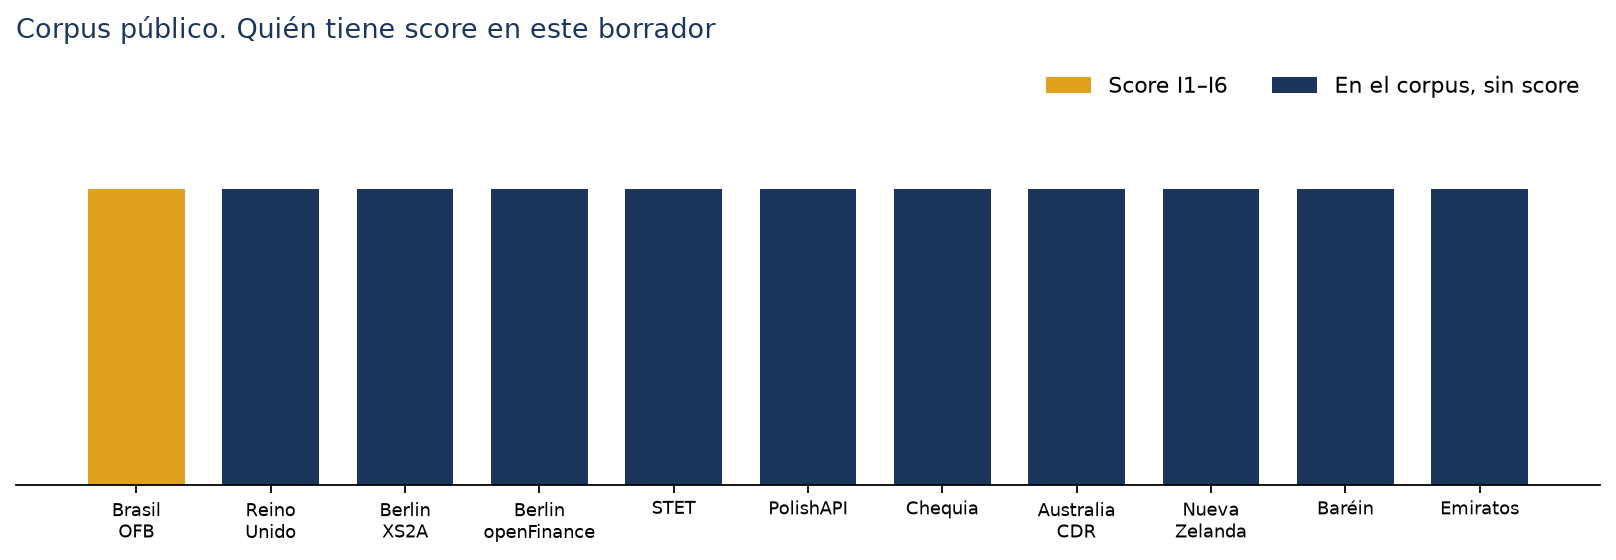
\includegraphics[width=\textwidth]{grafico-corpus}
  \caption{Once contratos públicos. Solo Open Finance Brasil tiene score en este borrador}
  \label{fig:corpus}
\end{figure}

\begin{figure}[ht]
  \centering
  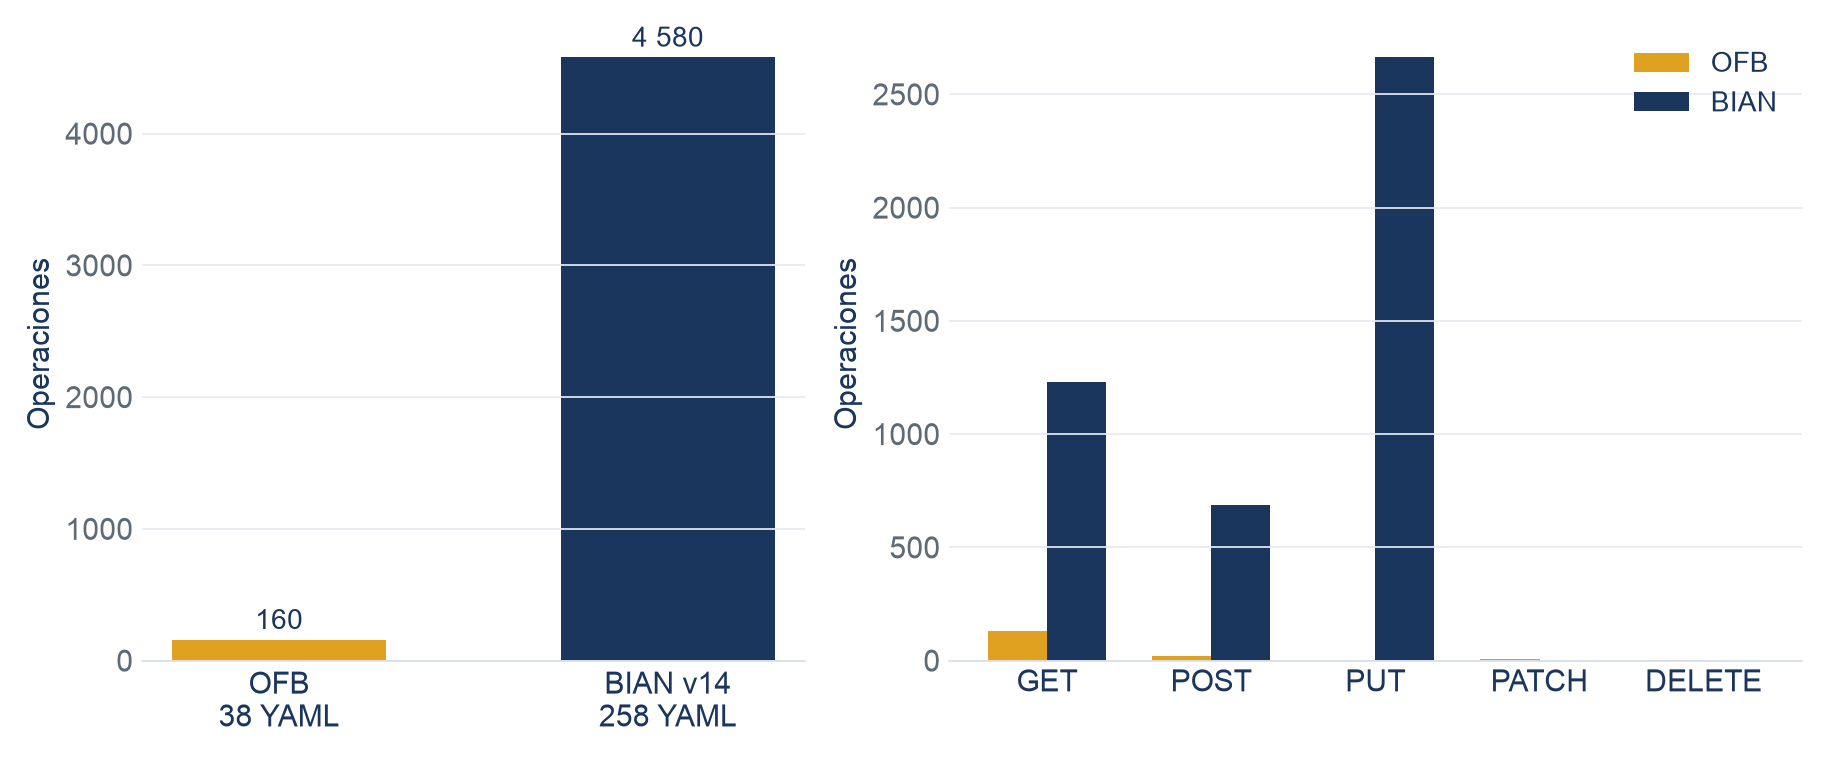
\includegraphics[width=0.92\textwidth]{grafico-fuentes}
  \caption{Operaciones del piloto ya parseado: 160 en OFB y 4\,580 en BIAN v14. OFB es sobre todo GET. BIAN es sobre todo PUT}
  \label{fig:fuentes}
\end{figure}

Tres archivos más se bajaron y no entran a la muestra de score. Son de un banco, o de un solo recurso, no un estándar de cuentas y pagos: VÚB (Eslovaquia, su XS2A), K\&H (Hungría) y el Swagger de cajeros de la CNBV (México, \texttt{GET /atms}). El YAML del Account Aggregator de ReBIT (India, 2.1.0) describe el flujo del agregador. No es el contrato de cuentas de un banco. Queda en el inventario.

FDX, el estándar de Estados Unidos y el que Canadá designó, no se baja sin registro. Italia (CBI Globe) deja el OpenAPI detrás de un portal. Chile, Colombia, Perú, Singapur, Hong Kong, Japón y el resto de la nota de fuentes tienen regla o PDF. No entran al parser. Los agregadores comerciales (Plaid, Tink, TrueLayer y los del Golfo) no son el estándar.

\begin{table}[ht]
  \centering
  \caption{Adquisición ya parseada: piloto Open Finance Brasil $\times$ BIAN v14}
  \label{tab:datos}
  \begin{tabular}{@{}lrrr@{}}
    \toprule
     & Open Finance Brasil & BIAN v14.0.0 & Total \\
    \midrule
    Contratos & 38 & 258 & 296 \\
    Operaciones & 160 & 4\,580 & 4\,740 \\
    \bottomrule
  \end{tabular}
\end{table}

Los YAML de Open Finance Brasil vienen de \url{https://github.com/OpenBanking-Brasil/openapi}. La muestra de score son siete instancias, no el producto 38$\times$258 y no el resto del corpus. I1 con I2, e I3a con I3b, comparten YAML. No son siete observaciones independientes.

\begin{table}[ht]
  \centering
  \caption{Muestra de score}
  \label{tab:muestra}
  \small
  \begin{tabular}{@{}llp{0.28\textwidth}p{0.32\textwidth}@{}}
    \toprule
    ID & OFB & BIAN & Para qué está \\
    \midrule
    I1 & accounts 2.4.2 & Savings Account & Par de cuentas \\
    I2 & el mismo YAML & Current Account & El mismo contrato, otro dominio \\
    I3a & opendata-accounts 1.0.1 & Savings Account & Cuentas en datos abiertos \\
    I3b & el mismo YAML & Current Account & El mismo contrato, otro dominio \\
    I4 & payments 4.0.0 & Payment Order Initiation & Pagos \\
    I5 & automatic-payments 2.0.0 & Payment Order Initiation & Pagos automáticos \\
    I6 & enrollments 2.1.0 & Payment Order Initiation & Control negativo. FIDO, no una orden de pago \\
    \bottomrule
  \end{tabular}
\end{table}

La firma de OE1 compara operaciones y esquemas extraídos contra lo que el YAML declara. Los 296 quedaron firmados. Las propiedades se cuentan en \texttt{properties} directas. No copiamos tags \texttt{CR} ni \texttt{BQ} al YAML de OFB.

\subsection{StructuralScore}

Un candidato entra si el Jaccard del nombre llega a 0,40, o el último tramo de la ruta toca un token del recurso del Service Domain, o el verbo es el mismo y el Jaccard del nombre llega a 0,25. Dentro del par el verbo suma 1 si es idéntico y 0,5 si los dos son de lectura o los dos son de escritura. Esa media no abre la puerta.

\[
e_{\mathrm{pair}} = 0{,}40\cdot\mathrm{nombre} + 0{,}25\cdot\mathrm{ruta} + 0{,}20\cdot\mathrm{verbo} + 0{,}15\cdot\mathrm{profundidad}
\]

El verbo vale 1 si es el mismo, 0,5 si ambos son de lectura o ambos de escritura, y 0 si cruzan. GET y PUT pueden emparejarse.

\begin{figure}[ht]
  \centering
  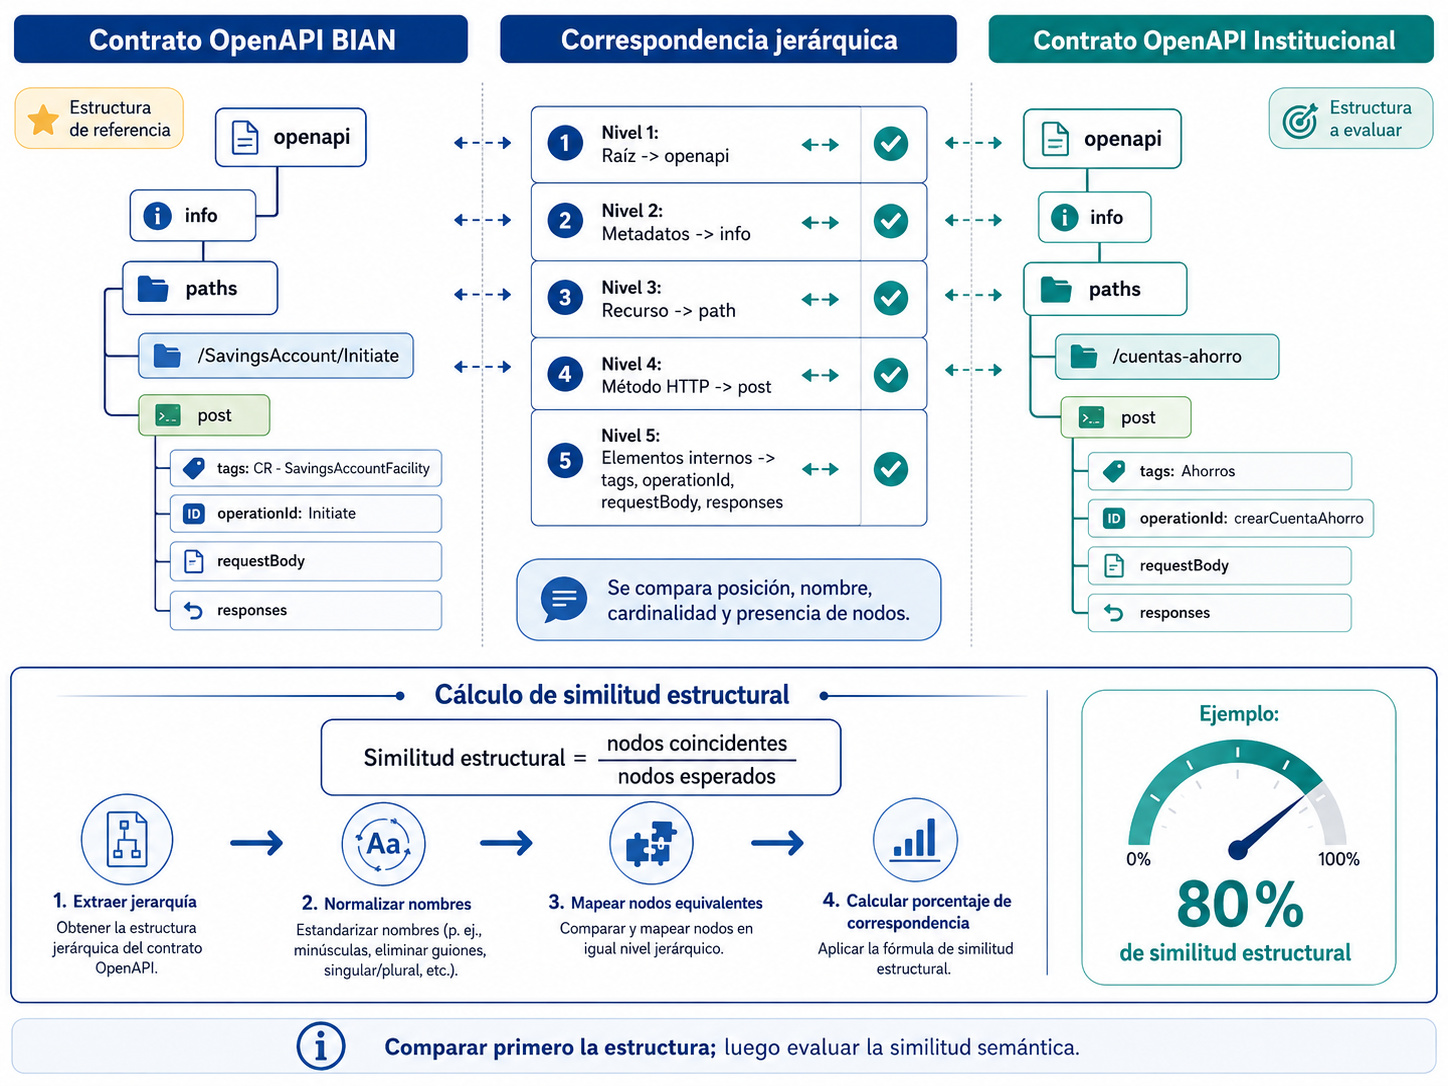
\includegraphics[width=0.92\textwidth]{Figura_07_StructuralScore}
  \caption{Correspondencia que entra en el StructuralScore}
  \label{fig:estructural}
\end{figure} El greedy asigna cada operación una sola vez. La operación OFB sin par entra como 0. E es la media de $e_{\mathrm{pair}}$ sobre todas las operaciones OFB.

\subsection{SemanticScore}

S v0, solo en los pares, es la media de dos cosas: el Jaccard de los tokens y el coseno TF-IDF. Sin GPU. El texto de OFB está en portugués y el de BIAN en inglés. Por eso el S léxico se queda cerca de cero.

S v1 usa \texttt{sentence-transformers/paraphrase-multilingual-MiniLM-L12-v2}, ya entrenado, sin fine-tuning. El vector se normaliza y el coseno es el producto punto. S v1 es la media de esos cosenos sobre los mismos pares. Los cortes 0,45 / 0,55 / 0,65 se guardan como sensibilidad. No recortan el S oficial.

\subsection{CoverageScore y AlignmentScore}

C es la fracción de tags \texttt{CR} y \texttt{BQ} del Service Domain que recibieron al menos un par.

\begin{figure}[ht]
  \centering
  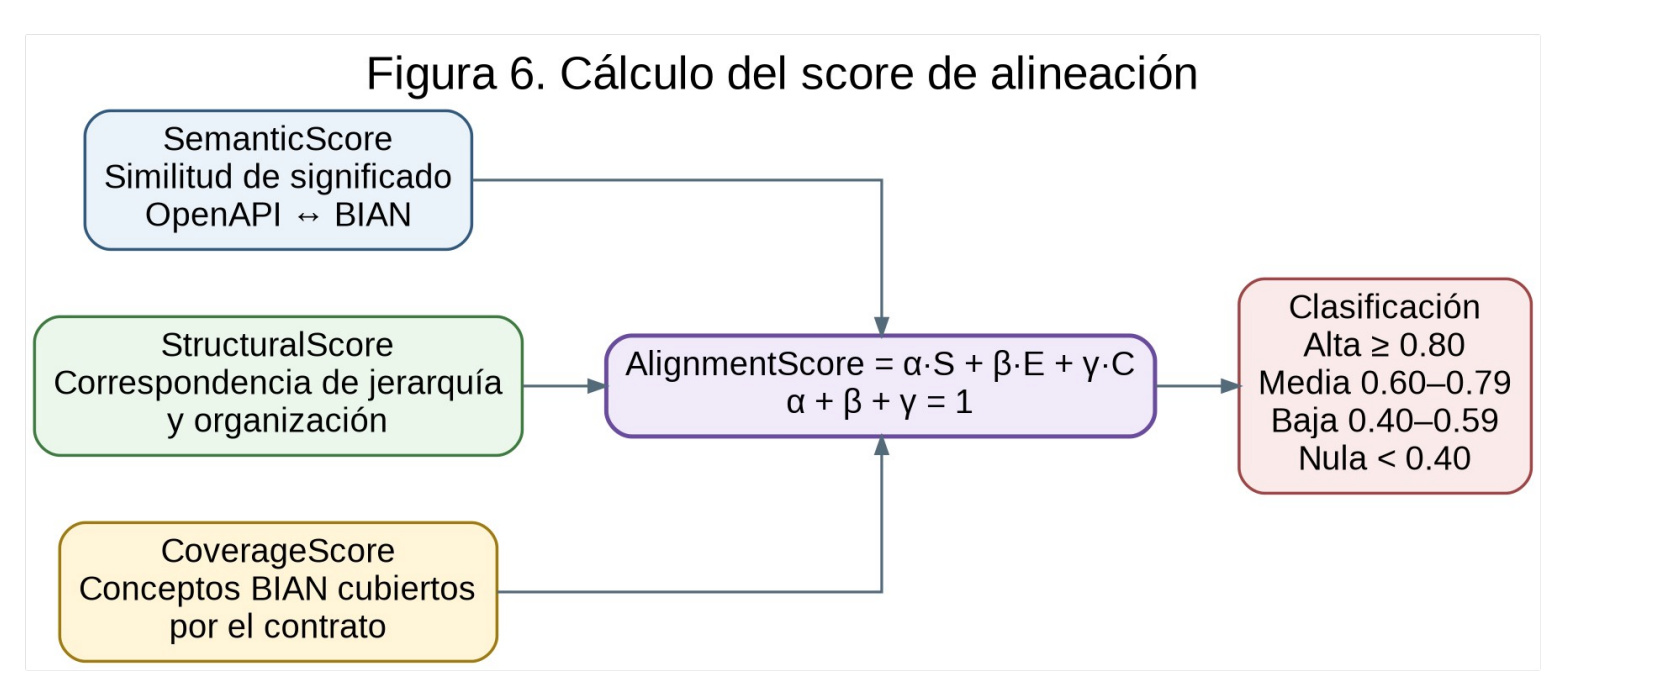
\includegraphics[width=0.85\textwidth]{Figura_03_AlignmentScore}
  \caption{S, E y C entran en el AlignmentScore}
  \label{fig:score}
\end{figure}

AlignmentScore oficial $= (S + E + C) / 3$. La sensibilidad, sin cambiar el número oficial, usa $(0{,}50,\ 0{,}30,\ 0{,}20)$ y $(0{,}20,\ 0{,}50,\ 0{,}30)$.

\begin{table}[ht]
  \centering
  \caption{Niveles del AlignmentScore}
  \label{tab:niveles}
  \begin{tabular}{@{}ll@{}}
    \toprule
    Nivel & Corte \\
    \midrule
    Alta & 0,80 o más \\
    Media & 0,60--0,79 \\
    Baja & 0,40--0,59 \\
    Nula & menor que 0,40 \\
    \bottomrule
  \end{tabular}
\end{table}

\section{Análisis de los datos y resultados}

S de la tabla es MiniLM. E y C son los del matching v0. El detalle está en el archivo \path{results/matching_s1/COMPARACION_V0_V1.md} del piloto.

\begin{table}[ht]
  \centering
  \caption{Scores preliminares de I1 a I6}
  \label{tab:scores}
  \small
  \begin{tabular}{@{}lrrrrrrl@{}}
    \toprule
    ID & S léxico & S MiniLM & E & C & Score v0 & Score v1 & Nivel \\
    \midrule
    I1 & 0,01 & 0,56 & 0,35 & 0,40 & 0,26 & 0,44 & Nula $\to$ Baja \\
    I2 & 0,01 & 0,53 & 0,47 & 0,50 & 0,33 & 0,50 & Nula $\to$ Baja \\
    I3a & 0,00 & 0,45 & 0,56 & 0,20 & 0,25 & 0,41 & Nula $\to$ Baja \\
    I3b & 0,00 & 0,46 & 0,56 & 0,20 & 0,25 & 0,41 & Nula $\to$ Baja \\
    I4 & 0,00 & 0,52 & 0,29 & 0,25 & 0,18 & 0,35 & Nula $\to$ Nula \\
    I5 & 0,03 & 0,59 & 0,32 & 0,50 & 0,28 & 0,47 & Nula $\to$ Baja \\
    I6 & 0,00 & 0,00 & 0,00 & 0,00 & 0,00 & 0,00 & Nula $\to$ Nula \\
    \bottomrule
  \end{tabular}
\end{table}

Pares que armó el greedy, sobre operaciones OFB: I1 4/6, I2 5/6, I3a 2/2, I3b 2/2, I4 3/6, I5 4/7, I6 0/8.

Los dos juegos de pesos, $(0{,}50,\ 0{,}30,\ 0{,}20)$ y $(0{,}20,\ 0{,}50,\ 0{,}30)$, dejan el nivel oficial igual en las siete instancias. En I4 el peso mayor sobre S da 0,399 y sigue en Nula. El S de la tabla es la media y no se recorta. Si pusiéramos en cero los pares con coseno bajo 0,45, I3a bajaría a 0,340 e I3b a 0,341, de Baja a Nula. Con el corte 0,55, I1 bajaría a 0,394, también Nula. Esos cortes son una bandera. No cambian el score de la tabla.

\begin{figure}[ht]
  \centering
  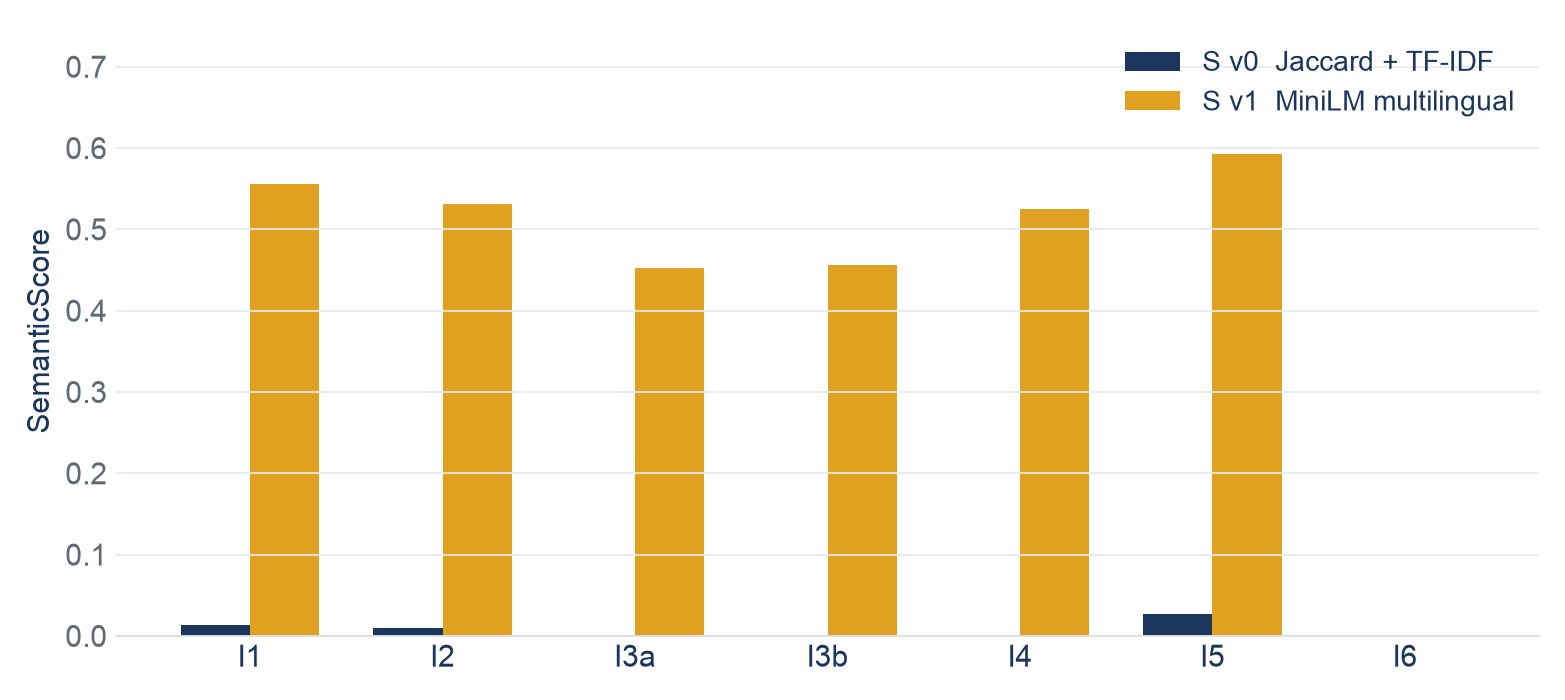
\includegraphics[width=0.88\textwidth]{grafico-semantico}
  \caption{SemanticScore. El léxico queda en el piso. MiniLM sube I1 a I5 y deja I6 en cero}
  \label{fig:semantico}
\end{figure}

\begin{figure}[ht]
  \centering
  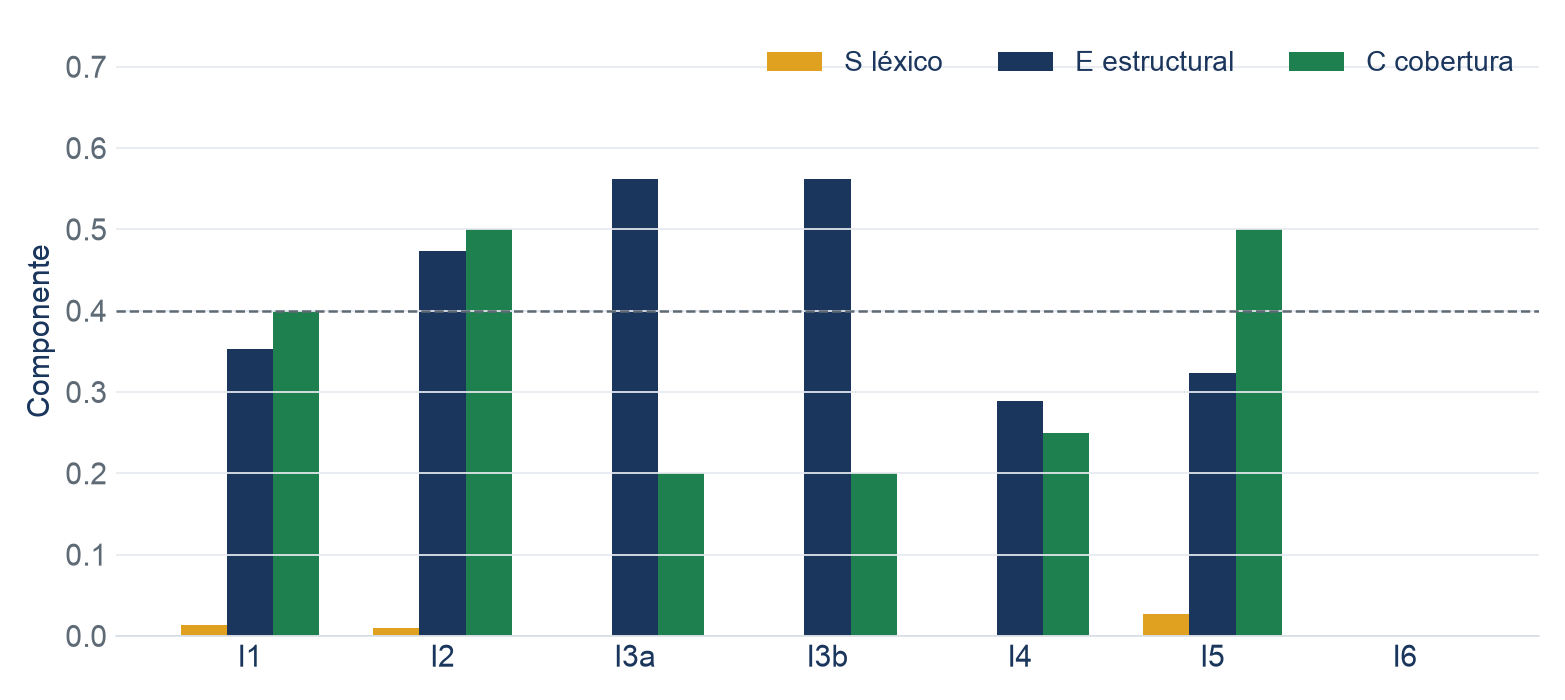
\includegraphics[width=0.88\textwidth]{grafico-sec}
  \caption{S léxico, E y C del matching v0. La línea punteada es 0,40}
  \label{fig:sec}
\end{figure}

\begin{figure}[ht]
  \centering
  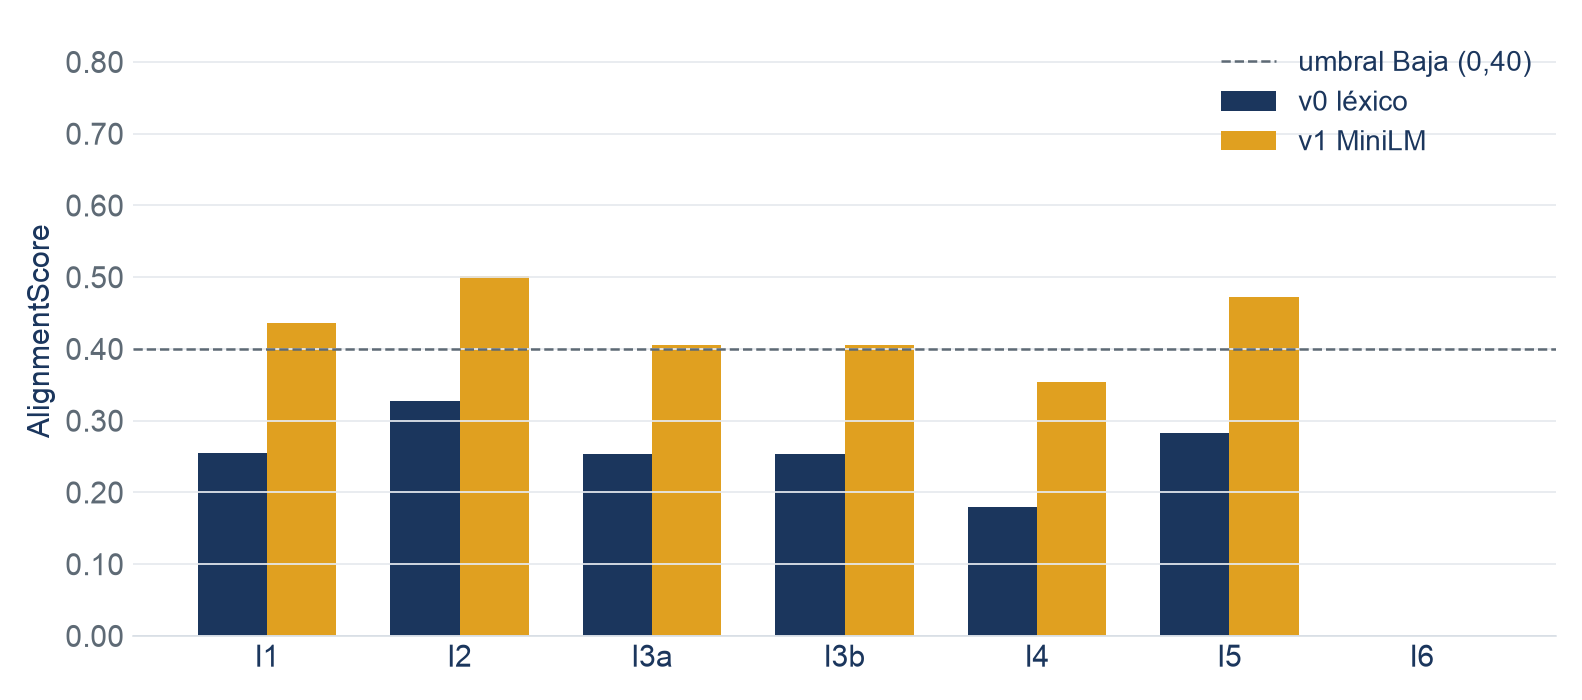
\includegraphics[width=0.88\textwidth]{grafico-alignment}
  \caption{AlignmentScore v0 y v1. I6 no tiene barra. La línea punteada es el corte de Baja}
  \label{fig:alignment}
\end{figure}

El catálogo extra (préstamos, tarjetas, inversiones) no entra en $n = 7$. El gráfico siguiente es el score v0, el léxico, no el MiniLM.

\begin{figure}[ht]
  \centering
  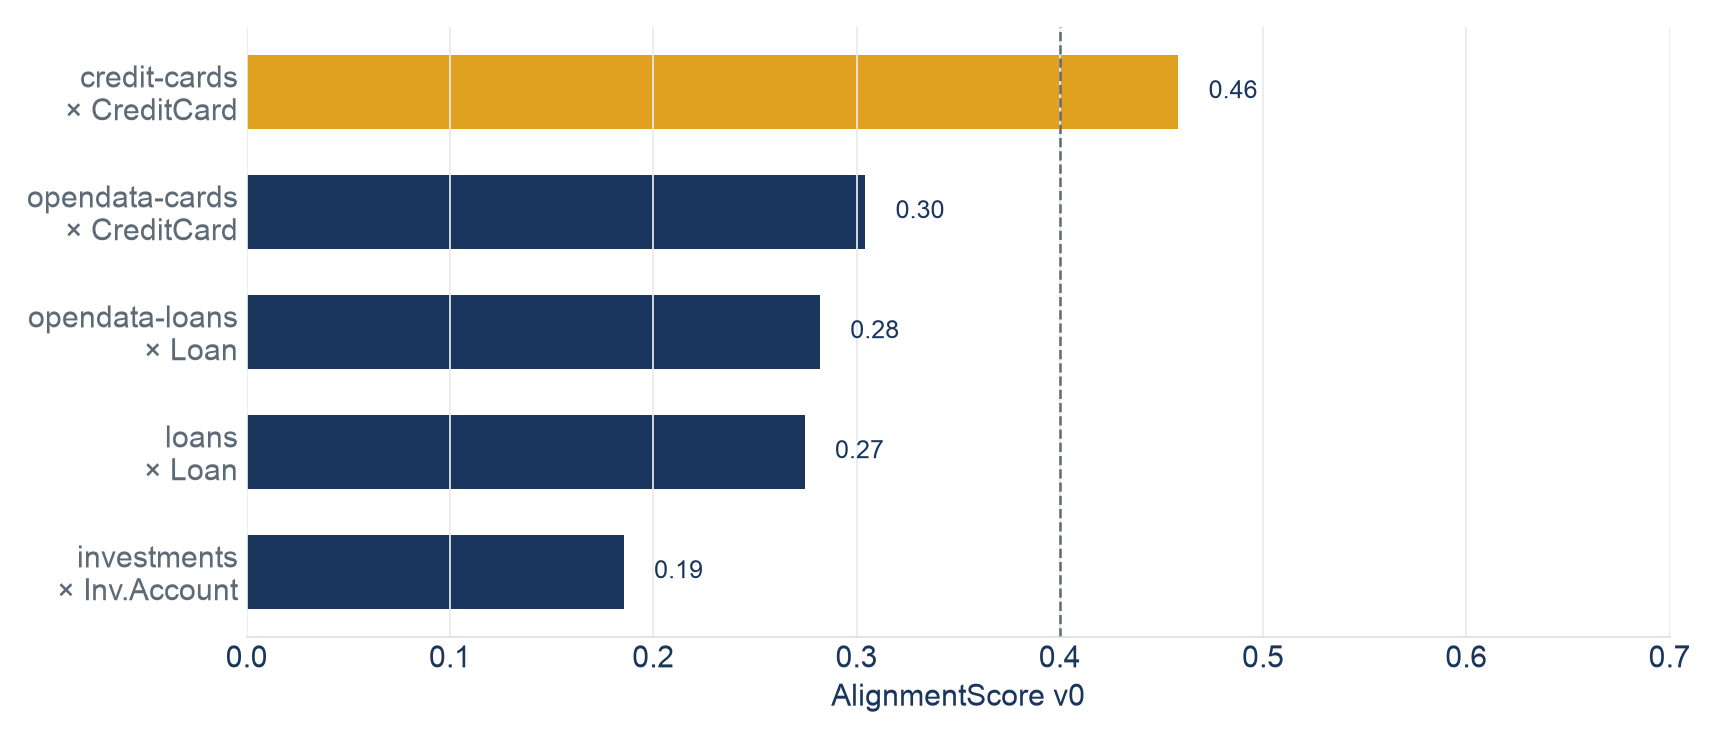
\includegraphics[width=0.82\textwidth]{grafico-catalogo}
  \caption{Catálogo v0, fuera de la muestra oficial. Solo credit-cards pasa de 0,40, y es el score léxico}
  \label{fig:catalogo}
\end{figure}

Nadie llega a Alta. Nadie llega a Media. Cinco instancias pasan de Nula a Baja cuando S deja de ser léxico. I4 se queda en Nula: S sube a 0,52, y E (0,29) con C (0,25) bajan la media a 0,35. I6 se queda en cero. No hubo par. El control negativo no inventó una correspondencia.

\section{Discusión e interpretación de los resultados}

El S léxico entre 0,00 y 0,03 no dice que las cuentas no se parezcan a Savings Account. Dice que \texttt{conta} y \texttt{SavingsAccountFacility} no comparten tokens. MiniLM, entrenado en varios idiomas y sin ajuste nuestro, sube S a la banda 0,45--0,59 en I1--I5 y lo deja en 0 en I6. El léxico es el piso. MiniLM es el S que reportamos en esta corrida.

El puntaje E no exige el mismo verbo. Si los dos son de lectura, o los dos de escritura, esa pieza vale 0,5. Si exigiéramos el verbo idéntico en el puntaje, OFB (casi todo GET) contra BIAN (casi todo PUT de ciclo de vida) caería por una convención de interfaz. Aun así E queda bajo en pagos: I4 en 0,29 e I5 en 0,32. De 6 y 7 operaciones OFB, el greedy sostiene 3 y 4 pares. Las que sobran entran como 0 en la media.

C cuenta otra cosa: cuántos tags \texttt{CR} y \texttt{BQ} del dominio recibieron par. En opendata-accounts, C $= 0{,}20$. El YAML abierto no cubre el desglose de behaviors de Savings Account.

En I1 el greedy arma cuatro pares de seis. \texttt{GET /accounts} cae en \texttt{Retrieve} (coseno 0,57), sobre Savings Account Facility. \texttt{GET /accounts/\{accountId\}}, que pide la identificación de la cuenta, cae en \texttt{RetrieveCharge} (0,59), una comisión. Los saldos caen en \texttt{RetrieveDeposit} (0,56). Las transacciones caen en \texttt{RetrieveInterest} (0,51). Quedan sin par \texttt{transactions-current} y \texttt{overdraft-limits}. C $= 0{,}40$ es 4 de 10 tags, y tres de esos cuatro son Charge, Interest y Deposit.

En I4, \texttt{POST /pix/payments} cae en \texttt{Initiate} (0,61). El GET de ese pago cae en \texttt{Retrieve} (0,47). El PATCH, cuyo texto es cancelar, cae en \texttt{Update} (0,49). Los tres consentimientos quedan sin par. C $= 0{,}25$ es un tag de cuatro: solo Payment Order Initiation Transaction. Compliance, Confirmation y Order Initiation no recibieron par.

I1 e I2 son el mismo \texttt{accounts} 2.4.2 contra dos dominios. Lo mismo I3a e I3b. La muestra de score es siete instancias y menos de siete contratos.

Los niveles no están calibrados. Hasta que etiquetemos match o no-match por recurso de negocio, y el asesor adjudique el desacuerdo, no hay kappa ni F1. Un verdadero positivo será un par del greedy que confirmemos. Un falso positivo, un par que rechacemos. Un falso negativo, un par nuestro que el greedy no armó.

\section{Estimación del impacto de la solución}

No estimamos VAN, TIR ni un costo evitado. No hay despliegue. Lo que el piloto ya cambia es la lectura del expediente de Open Finance Brasil: sin el encoder, las siete instancias quedan en Nula; con MiniLM, cinco pasan a Baja y el control negativo sigue en cero. Ese salto es el efecto medible de esta corrida.

El corpus nuevo cambia la pregunta, no el número. Casi todos los estándares de la tabla del corpus están en inglés, igual que BIAN. El piso léxico de 0,00 a 0,03 puede ser el portugués del YAML brasileño y no el desajuste de negocio. Hasta que el mismo procedimiento corra sobre Reino Unido, Berlin Group, STET o Australia, no se sabe cuál de las dos cosas es. Esas corridas no están en esta tabla.

\section{Amenazas a la validez}

La interna: el parser no aplana \texttt{allOf}, y el S léxico se acerca a cero porque el YAML del piloto está en portugués. Por eso guardamos el S v0 como piso y el S v1 no reabre los pares. La externa: los cortes 0,80 / 0,60 / 0,40 son convención, y siete instancias no representan crédito, ni un banco emisor, ni el resto del corpus. De constructo: un AlignmentScore medio puede esconder un esquema mal emparejado que al negocio le importa. De conclusión: el reporte lleva la instancia junto al score. La etiqueta y el F1 cierran esa lectura. Hasta que existan, el nivel es una convención. I6 en cero no es esa etiqueta.
